\documentclass{sig-alternate-05-2015}
\usepackage{subscript}
\usepackage{tikz}
\usepackage{hyperref}
\usepackage{graphicx}
\usepackage{amsmath}

\graphicspath{ {./imgs/} }

\begin{document}

\title{Topic-zoomer: a URL categorization system}

\numberofauthors{2}
\author{
    \alignauthor
    Gianluca Bortoli\\
           \affaddr{DISI\,-\,University of Trento}\\
           \affaddr{Student id: 179816}\\
           \email{gianluca.bortoli@studenti.unitn.it}
    \alignauthor
    Pierfrancesco Ardino\\
           \affaddr{DISI\,-\,University of Trento}\\
           \affaddr{Student id: 189159}\\
           \email{pierfrancesco.ardino@studenti.unitn.it}
    }
\maketitle


\begin{abstract}
Smartphones and tablets pervade our lives on a daily basis and people use them in most curious ways.\\ 
The key idea behind this work is to take advantage of the traffic they generate while they are connected to the Internet, extracting \emph{topics} from what people search on the web with their mobile devices. This use case provides also the geographical coordinates of the users based on the telephone cell they are connected to.\\
For the purpose of this work the approximate location of the cell is enough, even thoug it implicitly defines a limit on the precision while selecting an area inside a map.\\
This paper presents Topic-zoomer, a URL categorization system built upon Apache Spark.
\end{abstract}


\printccsdesc
\keywords{Big data, Data mining, URL categorization, topic extraction, geolocalized URLs, Latent Dirichlet Allocation}


\section{Introduction}
Extracting topics from a text is a very common goal nowadays in Big Data and the problem of categorizing URLs is highly connected to it.\\
Generally speacking, the main aim is to find what a set of texts is talking about. Applying this reasoning to a more specific problem, Topic-zoomer is able to find the topics on a subset of the initial dataset, based on the documents' geographical location.\\
The tool starts from a set of geotagged URLs and is able to restrict its search space only to the web pages lying inside a certain geographical region. In this way it can discover what the pages in that spacific area are talking about.\\
This work can be employed in many different fields. For example it can be utilized to see what people are going to do in the future based on their web searches. Moreover it can be useful for public institutions such as municipalities: they could understand the citizens' needs in order to improve the functionality of the city's facilities and their territory coverage.\\
However, the main problem of a real-life usage of this kind of analysis can be the data source. Internet Service Providers (ISPs) can easily extract and provide geotagged URLs based on the HTTP requests passing through their routers. Furthermore the anonimity of the users generating such traffic must be preserved.\\
This kind of problems is a challange for traditional programming paradigms, since the amount of data can be huge and may also involve straming  processing. Big Data platforms and frameworks perfectly suit this amount of work that cannot fit in a single machine and has to scale as the input size increases. Thus employing an engine for large-scale and distributed data processing is certainly not an option if a system is thought to be used on real data.        


\section{Related work}
URL categorization is a task that many people and companies are addressing in the last few years, pushing even to the categorization of the whole World Wild Web. Some of the ones involved in this kind of analysis are Cyren\footnote{\url{http://www.cyren.com/url-category-check.html}} and BrightCloud\footnote{\url{https://www.brightcloud.com/tools/change-request-url-categorization.php}}. Moreover, a huge number academic researches have been published and also some patents\footnote{\url{https://www.google.com/patents/US8078625}} have been filed on the subject.\\
However the specific case of geotagged URLs has not raised so much interest neither in the academic nor in the developer communities.


\section{Problem definition}
The task Topic-zoomer aims to solve can be better described starting from its \emph{input} and \emph{output} data.\\
The \emph{input} is a CSV file containing rows of the following form:
\begin{equation}\label{dataset}
    <latitude,\,longitude,\,\{url0\,|url1\,|...\,\}\,>
\end{equation}
The text of the pages pointed by the URLs is analized in order to identify the topics that represented as a vector of words that very often appear togheter.\\
Let \emph{A} be an algorithm to compute such topics (eg. TF/IDF, frequent itemset or LDA; see Section \ref{algorithmSelection} for a more comprehensive description), the algorithm \emph{L} gives as a result the topics of the dataset in general.\\
\emph{L} also allows the user to restrict the search in the dataset using the following parameters:
\begin{itemize}
    \item \emph{A}: the map area identified by top-left and bottom-right corners. This is the region of interest for retrieving the topics. 
    \item \emph{S}: the size of the grid to be created inside the area \emph{A} (ie. the square side length).
    \item \emph{k}: the number of topics to search inside each square of the grid.
\end{itemize}
In this way \emph{A} is divided into squares of size $S \times S$ and the \emph{k} topics are identified inside each such square.


\section{Solution}
This section describes in detail all the steps needed to realize this tool, from the initial web page download to the map-reduce operations taken by Spark. The order in which they are presented reflects the one followed during the experiments.
\subsection{Data collection and preprocessing}\label{preprocessing}
The first task was to transform an initial dataset with the form shown in \ref{dataset} into another one of the form
\begin{equation}\label{datasetClean}
    <latitude,\,longitude,\,page\_text\,>
\end{equation}
A \emph{crawler} has been written in order to follow all the links and download the web pages. This may seem a trivial operation at a first glance. However the initial dataset contained a lot of URLs pointing to images, videos, configuration files for mobile phones applications and many other elements that are far from being a text web page. To retrieve only sensible information, the crawler rejects all the requests not containing \emph{text/html} in the responses' headers. This is the one which is usually populated by a web server when a client visits one of its pages. Last but not least, the crawler uses multiple processe to minimize the download time. Multiple processes are preferred to multiple threads because the crawler is written in Python and this language is known to be subject to the Global Interpreter Lock\cite{gil} (GIL).\\
Finally a new CSV file containing rows as described in \ref{datasetClean} is generated.
\subsection{Algorithm selection}\label{algorithmSelection}
After downloading the web pages, the Spark pipeline is ready to run on the clean dataset.\\
Among all the ways to extract topic, the \emph{Latent Dirichlet Allocation}\cite{lda} (LDA) algorithm is chosen as \emph{L} to find the topics of the dataset in general. LDA is a generative and probabilistic model for collections of discrite data such as text corpora. It is a Bayesian hierarchical model, where each topic is modeled over an underlying set of topic probabilities. LDA is a good candidate when choosing between different methods to classify text. This work uses the implementation inside the Spark MLlib for the inference step.\\
From a higher perspective LDA can be seen as a clustering technique, whose goal is to divide the document corpora given as input into \emph{k} clusters, which are the topics to be retrieved from the text.
\subsection{Spark pipeline}
Spark is a framework that allows to write parallel applications in many languages using the map-reduce paradigm. Python\footnote{For the seek of completeness, Python3 with version \textless\,3.6 is used.} is chosen for the development of this work in order to focus on the real data manipulation and analysis rather than continuously dealing with language-specific issues. Moreover, the Python interface for Spark is very concise and makes the application maintainable in long-term projects.\\
The pipeline of operations is composed as follows:
\begin{itemize}
    \item provide Topic-zoomer with the parameters \emph{A}, \emph{S} and \emph{k}.
    \item read the dataset (in CSV format) generated by the pre-processing phase described in Section \ref{preprocessing}.
    \item divide \emph{A} into squares with dimension $S \times S$ (ie. compute the inner grid).
    \item filter the input data to retrieve only the points lying inside each square of the grid. At the same time a dataframe for each one of them is created.\\
    Next take the following steps for each square:
    \begin{itemize}
        \item remove punctuation and stopwords for the language of interest\footnote{In this specific case, italian, english and german stopwords are removed due to the source of the dataset used for the experiments.} in order not to consider the most common words in the sentences.
        \item convert every text into vectors of token counts. This step is needed for preparing the dataframes with a format suitable for the LDA algorithm.
        \item train the LDA model with the proper \emph{k} parameter.
        \item collect the results from HDFS.
    \end{itemize}
\end{itemize}
The choice of creating one dataframe for each $S \times S$ square in the grid allows to fully exploit the parallelism offered by Spark. In this way the master node always has data to send to the workers to keep them busy until the end of the computation. This approach should optimize the CPU usage in the worker nodes, taking advantage of the full computation power made available by the cluster.
\subsection{Avoiding recomputation}\label{avoidingRecomputation}
One of the main issues these kind of tools has to face is the overall time to answer a user query.\\
The main idea bihind this feature can be better explained referring to Figure \ref{recomputation}. The top-left square represents an area (\emph{oldA}) the tool already computed the topics for in a previous run, while the bottom-right one a new area (\emph{newA}) of interest. It would be useful not to recompute the topics for the whole \emph{newA}, since \emph{oldA} and \emph{newA} have a part in common (ie. \emph{commonA}, the blue square). This can be achieved trining the LDA model only on the white area without including the \emph{commonA} part, as it would happen without this feature. As the blue region becomes bigger, the whole run of the tool will take less time with respect to a naive implementation. This improvement is due to the fact that \emph{newA} contains less points and thus the underlying LDA model will be trained with fewer items.\\
When dealing with the scenarios mentioned above, the overall result returned for \emph{newA} must take the topics coming from \emph{commonA} into account. The LDA returns as output a list containing the topics in the following form:
\begin{equation}
    \begin{split}
        [\,probability_0,\,topic_0\,] \\
        \cdots \\
        [\,probability_k,\,topic_k\,]
    \end{split}
\end{equation}
The lists computed starting both from \emph{newA} and \emph{commonA} have be merged, producing a single topic lisk of length \emph{k} as output. The merging procedure is implemented as follows: the list produced starting from \emph{newA} is considered as is, while the probability values in the list produced starting from \emph{oldA} are multiplyed by a factor \emph{f} computed as shown in Equation \ref{factor}.
\begin{equation}\label{factor}
    f = \frac{area_{commonA}}{area_{oldA}}
\end{equation}
In this way \emph{f} weights the topics previously found for \emph{oldA} with respect to the size of \emph{commonA} when computing the tipics starting from \emph{newA}. To retrieve the final output all the topics are ordered by decreasing probability values and  the first \emph{k} of them are taken.

\begin{figure}[t]
  \center{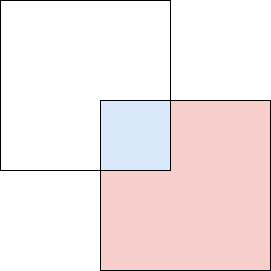
\includegraphics[width=0.22\textwidth]{recomputationSchema.png}}
  \caption{Idea to avoid useless recomputation.}
  \label{recomputation}
\end{figure}

\section{Architecture}
Apache Spark and all the other big data distributed frameworks are thought to be set up in a cluster of machines. In this way it is possible to exploit its distributed mode and all the computation power from the worker nodes. To achive this Google Dataproc\footnote{\url{https://cloud.google.com/dataproc/}} on the Google Compute Engine\footnote{\url{https://cloud.google.com/compute/}} (GCE) is used to provision and setup a Spark cluster.\\

One of the main focuses of this work is the \emph{scalability} of this piece of software. To see if Topic-zoomer really succeedes in it, a pseudo-distributed Spark cluster may produce completely misleading or even wrong results. Thus a platform providing highly performing vistual machines (VMs) was mandatory.\\
The cluster used for the experiments described in Section \ref{experiments} is composed as shown in Table \ref{cluster}. Google Dataproc makes use of Apache YARN and provides access to an Hadoop Distributed File System (HDFS) shared among all the nodes.\\
Moreover it is fully integrated with Google Cloud Storage (GCS), a flexible, scalable and distributed storage for VM instances. All the input data presented in Table \ref{datasets} are stored in a shared bucket on GCS to allow every node in the cluster to mount it through its FUSE\footnote{\url{https://www.kernel.org/doc/Documentation/filesystems/fuse.txt}} adapter.  

\begin{table}[]
    \centering
    \caption{GCE cluster node characteristics.}
    \label{cluster}
    \begin{tabular}{lllll}
    \hline
    Node   & Number & vCPUs & RAM (GB) & SSD (GB) \\
    \hline
    master & 1      & 1     & 3.75     & 500      \\
    worker & 3      & 2     & 7.50     & 500     
    \end{tabular}
\end{table}


\section{Experiments}\label{experiments}
The experiments shown in this section focus on a quantitative rather than a qualitative performances of the system. Measuring timings is a way to provide unbiased results regarding the real its ability to scale and respond to queries.\\
Some performance measuser has to be computed in order to measure how Topic-zoomer behaves under different scenarios. In order to better understand the results, Table \ref{datasets} should be taken as reference. It displays the composition and the sizes of the input data used throughout all the experiments. As it is possible to see, the whole dataset (i.e. \emph{input\_100}) is split into different parts with increasing size in order to be able to run the experiments with different volumes of data.

\begin{table}[]
    \centering
    \caption{Input data description.}
    \label{datasets}
    \begin{tabular}{llll}
    \hline
    ID         & \% of whole dataset & \# of lines & Size (MB) \\
    \hline
    input\_15  & 15                  & 52623       & 11        \\
    input\_30  & 30                  & 105246      & 21        \\
    input\_45  & 45                  & 157872      & 30        \\
    input\_60  & 60                  & 210495      & 40        \\
    input\_75  & 75                  & 263118      & 54        \\
    input\_90  & 90                  & 315741      & 63        \\
    input\_100 & 100                 & 350826      & 69       
    \end{tabular}
\end{table}

The four different test procedures are thought to highlight how the tool behaves from different point of views, especially from the ones of scalability and best/worst case.\\
The \emph{time} it takes to display a result is very important when dealing with this type of systems. Therefore this can be considered as the main measure to state how well such systems perform.\\
Moreoreover a single run for a test cannot be blindly trusted. The same algorithm with the same input may take very different amount of time to output a result due to cold start issues with the Spark cluster, especially when dealing with relatively small datasets. Thus all the charts presented in this section are generated after repeating every test 4 times. The number of repetitions represents a tradeoff between the time taken to run the experiment and the number of runs that would be needed to retrieve statistically significant timing result. As a result, the average among the 4 identical runs is computed and shown as value for each one of them, while the red vertical bars show the difference between the best and the worst performing run.\\

The graph in Figure \ref{scalability} shows how Topic-zoomer scales with respect to the dataset size. The time in the \emph{y} axis is shown in \emph{logarithmic scale}, while the \emph{x} axis represents the percentage of the whole dataset used. It is clear how the time taken by the tool to infer the topics is not exponential in the size of the input data. Thus it is possible to state that Topic-zoomer scales properly and in a linear manner.  
Another important aspect while processing a large amount of data is to show the worst and the best case scenarios for the algorithm. The LDA algorithm is faster when deals with few points located inside the region selected by the user, because the underlying model to be trained is smaller.\\
Figure \ref{square} depicts how performances degrade increasing the size of the region selected. The time in the ordinate axis is always in logarithmic scale to allow a more direct interpretation of the chart. Moreover, in this experiment the grid size (i.e. the \emph{step}) is set to be equal to te one of the selected area \emph{A}. It is not surprising that the time trend in Figure \ref{square} is nearly the same as the one in Figure \ref{scalability}. This means that selecting bigger areas via the top-left and bottom-right corners is the equivalent of having a bigger input dataset.\\  
In addition, Figure \ref{step} shows the performance keeping the selected region unchanged, while the \emph{S} parameter describing the inner grid increases. For this experiment, the selected top-left and bottom-right corners formed a square whose side size is 5. The graph shows a huge increase increasing the grid size from 2 to 3 and from 3 to 4. Moreover, when the step \emph{S} is set to the size of the whole area \emph{A} the time taken to complete the topic extraction seems to decrease. This corroborates the idea that the selection of the \emph{S} parameter highly influences the computation time and that the worst case for the algorithm is when the grid size is set to the one of the side of \emph{A}.\\
Finally, Figure \ref{recomputation} highlights the effect of the method employed to avoid recomputation described in Section \ref{avoidingRecomputation} using the \emph{input\_15} dataset. The time in the \emph{y} axis is always plot in logarithmic scale. As it is possible to see, the time taken to complete the topic extraction decreases as the percentage of the \emph{commonA} area increases. This is clearly due to the smaller amount of points to be considered when training the LDA model. As a result, this method allows Topic-zoomer to run significantly faster even when dealing with rather small input data. 

\begin{figure}[t]
  \center{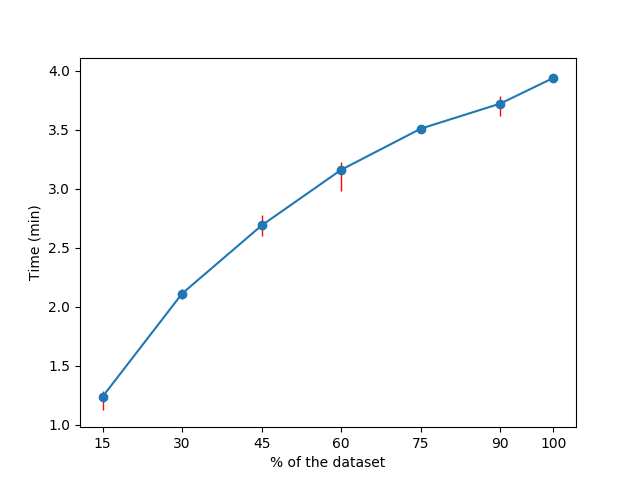
\includegraphics[width=0.5\textwidth]{scalability.png}}
  \caption{Scalability with different input size.}
  \label{scalability}
\end{figure}
\begin{figure}[t]
  \center{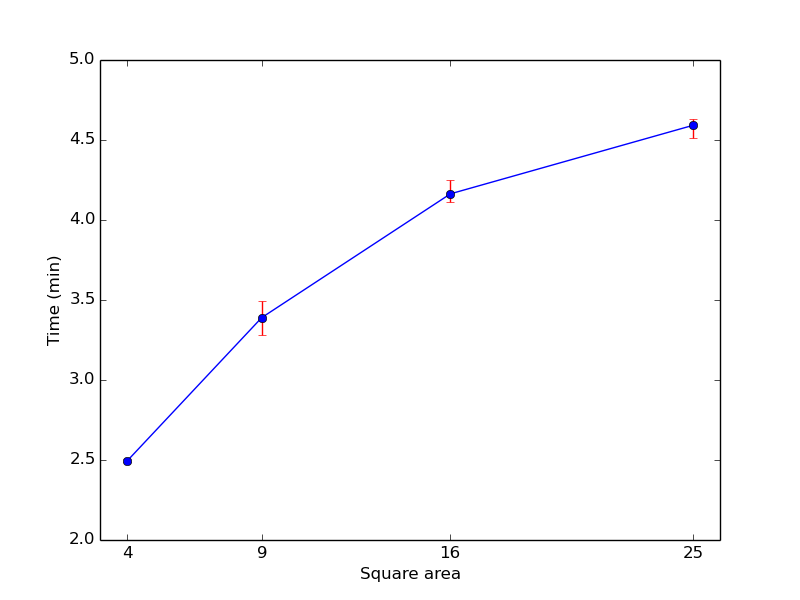
\includegraphics[width=0.5\textwidth]{increasing_square_size.png}}
  \caption{Performance with different area selections.}
  \label{square}
\end{figure}
\begin{figure}[t]
  \center{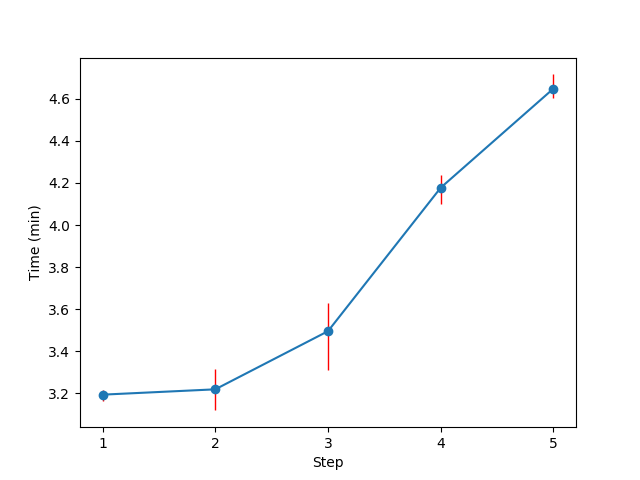
\includegraphics[width=0.5\textwidth]{increasing_step.png}}
  \caption{Performance with different grid size.}
  \label{step}
\end{figure}
\begin{figure}[t]
  \center{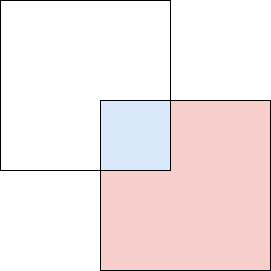
\includegraphics[width=0.5\textwidth]{recomputation.png}}
  \caption{Timings trend avioding recomputation.}
  \label{recomputation}
\end{figure}


\section{Conclusions and future work}
As described in Section \ref{experiments} quite good results are achieved from the scalability point of view. Even though the whole dataset size is not in the order gigabytes, the results are quite promising.\\
Further developments of this work may involve the creation of a graphical user interface (GUI), allowing the users to select the \emph{A} area and all the other parameters in a more convenient way. This can be done implementing a web UI showing a map of the territory we own data about (eg. Google Maps or OpenStreetMap) communicating with the Spark cluster backend. Once succeeded the results can be retrieved and shown to the user either as a table or as a chart.\\
Moreover some attention should be put to the visualization of the raw results of the Spark jobs. A neat and well organized presentation can improve not only immediate interpretation of the results, but also the usability of the tool for the general public.\\
Finally there is room for improvement in the part avoiding useless recomputation. For example it could be implemented using the map-reduce paradigm to further increment the performance from the scalability standpoint. 


%\end{document}  % This is where a 'short' article might terminate
%
% The following two commands are all you need in the
% initial runs of your .tex file to
% produce the bibliography for the citations in your paper.

\bibliographystyle{abbrv}
\bibliography{biblio}% biblio.bib is the name of the Bibliography in this case

% You must have a proper ".bib" file
%  and remember to run:
% latex bibtex latex latex
% to resolve all references
%
% ACM needs 'a single self-contained file'!
%

\end{document}
